\chapter{Metaheuristics}


Following the complexity of the problem, it may be solved by an exact method or an
approximate method. Exact methods obtain optimal solutions and guarantee
their optimality. Approximate (or heuristic) methods generate high quality
solutions in a reasonable time for practical use, but there is no guarantee of finding a global optimal solution \cite{Talbi2013}.


\begin{figure}[h]
\centering
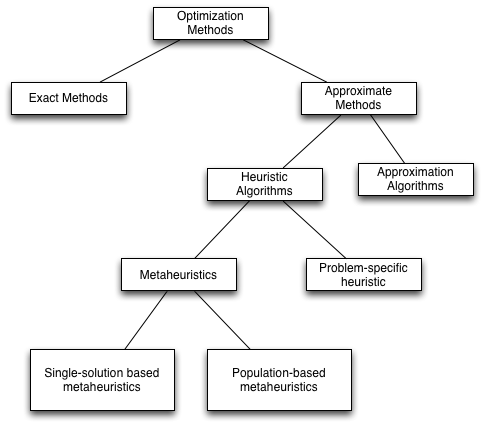
\includegraphics[width=0.7\textwidth]{./images/optimization.png}
\caption{Classical optimization methods \cite{Talbi2013}. }
\label{fig:optimization}
\end{figure}


In the computer science, the term metaheuristic is accepted for general techniques which are not specific to a particular problem. A metaheuristic is formally defined as an iterative generation process which guides a subordinate heuristic by combining intelligently different concepts for exploring and exploiting the search space \cite{raidl2010metaheuristic}. 

Metaheuristics are strategies that guide the search process to efficiently explore the search space in order to find optimal solutions. Metaheuristic algorithms are approximate and usually non-deterministic and sometimes incorporate mechanisms to avoid getting trapped in confined areas of the search space. There are different ways to classify and describe metaheuristic algorithm \cite{Blum2003}:

\begin{itemize}
\item Nature-inspired vs. non-nature inspired. There are nature-inspired algorithms, like Genetic Algorithms and Ant Algorithms, and non nature-inspired ones such as Tabu Search and Iterated Local Search. 

\item Population-based vs. single point search. Algorithms working on single solutions are called trajectory methods, like Tabu Search, Iterated Local Search and Variable Neighborhood Search. They all share the property of describing a trajectory in the search space during the search process. Population-based metaheuristics perform search processes which describe the evolution of a set of points in the search space.

\item One vs. various neighborhood structures. Most metaheuristic algorithms work on one single neighborhood structure. In other words, the fitness landscape topology does not change in the course of the algorithm. Other metaheuristics, such as Variable Neighborhood Search (VNS), use a set of neighborhood structures which gives the possibility to diversify the search by swapping between different fitness
landscapes.
\end{itemize}

\section{Single-Solution Based Metaheuristics}

While solving optimization problems, single-solution based metaheuristics
 improve a single solution. They could be viewed as "walks" through neighborhoods or search trajectories through the search space of the problem at hand.
 
 \begin{figure}[h]
\centering
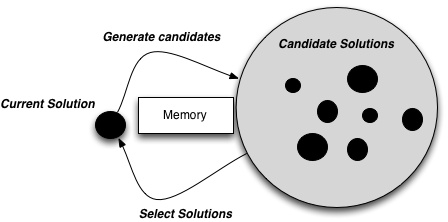
\includegraphics[width=0.6\textwidth]{./images/singlebased.png}
\caption{ Main principles of single-based metaheuristics.}
\label{fig:singlebased}
\end{figure}


\subsection{Neighborhood}

The definition of Neighborhood is a required common step for the design of any Single-Solution metaheuristic (S-metaheuristic). The neighborhood structure it is a important piece in the performance of an S-metaheuristic. If the neighborhood structure is not adequate to the problem,
any S-metaheuristic will fail to solve the problem. The neighborhood function N is a mapping: $ N : S \rightarrow N\textsuperscript{2} $ that assigns to each solution s of \textit{S} a set of solutions \textit{N(s)}$\subset$ S \cite{Talbi2013}.

The neighborhood definition depends  representation associated with the problem. For permutation-based representations, a usual neighborhood is based on the swap operator that consists in swapping the location of two elements $s_i$ and $s_j$ of the permutation \cite{Talbi2013}. The Fig. \ref{fig:sperneighborhood} presents a example where a set of neighbors is found by permutation. 


\begin{figure}[h]
\centering
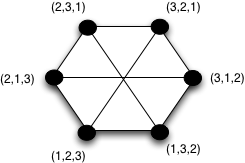
\includegraphics[width=0.5\textwidth]{./images/neighborhood.png}
\caption{ An example of neighborhood for a permutation \cite{Talbi2013}.}
\label{fig:sperneighborhood}
\end{figure}



Single-Solution Based Metaheuristics methods are characterized by a trajectory in the search space. Two common S-metaheuristics methods are Simulated Annealing and Tabu Search.


\subsection{Simulated Annealing}

Simulated Annealing (SA) is a randomized algorithm that tries to avoid being trapped in local optimum solution by assigning probabilities to deteriorating moves. The SA procedure is inspired from the annealing process of solids. SA is based on a physical
process in metallurgy discipline or solid matter physics. Annealing is the process of obtaining low energy states of a solid in heat treatment \cite{Jaziri2008}. 

The algorithmic framework of SA is described in Alg. \ref{sa}.  The algorithm starts by generating an initial solution in function \textit{GenerateInitialSolution()}. The initial temperature value is determined in function \textit{SetInitialTemperature()} such that the probability for an uphill move is quite high at the start of the algorithm. At each iteration a solution $\mbox{s}_1$ is randomly chosen in function \textit{PickNeighborAtRandom(N(s))}. If \textit{$\mbox{s}_1$} is better than \textit{s}, then \textit{$\mbox{s}_1$} is accepted as new current solution. Else, if the move from \textit{s} to \textit{$\mbox{s}_1$} is an uphill move, \textit{$\mbox{s}_1$}  is accepted with a probability which is a function of a temperature parameter \textit{Tk} and \textit{s} \cite{raidl2010metaheuristic}. 

\begin{algorithm}[h]
  \caption{Simulated Annealing Algorithm}\label{sa}
  \begin{algorithmic}[1]
    
    \State $s\gets GenerateInitialSolution()$
    \State $k\gets 0 $
    \State $Tk\gets SetInitialTemperature()$
    \While{termination conditions not met }
    \State $\mbox{s}_1\gets PickNeighborAtRandom(N (s))$
    \If{$(f(\mbox{s}_1)<f(s))$}
    \State $s\gets\mbox{s}_1$
    \Else $\;$ Accept $\mbox{s}_1$ as new solution with probability p($\mbox{s}_1|$Tk,s) 
    \EndIf
    \State $K\gets K+1$
    \State $Tk\gets AdaptTemperature()$
    \EndWhile
      
  \end{algorithmic}
\end{algorithm}

\subsection{Tabu Search}

Tabu Search (TS) is a metaheuristic that guides a local heuristic search procedure to explore the solution space beyond local optimal and search with short term memory to avoid cycles. Tabu Search uses a  tabu list to keep track of the last  moves, and don’t allow going back to these \cite{Glover1986}.

The basic idea of TS is the explicit use of search history, both to escape
from local minima and to implement a strategy for exploring the search space.
A basic TS algorithm uses short term memory in the form of socalled
tabu lists to escape from local minima and to avoid cycles \cite{Tobergte2013}.

The algorithmic framework of Tabu Search is described in Alg. \ref{tsa}.  The algorithm starts by generating an initial solution in function \textit{GenerateInitialSolution()} and the tabu lists are initialized as empty lists in function \textit{InitializeTabuLists($\mbox{TL}_1$,...,$\mbox{TL}_r$)}. For performing a move, the algorithm first determines those solutions from the neighborhood \textit{N(s)} of the current solution \textit{s} that contain solution features currently to be found in the tabu lists. They are excluded from the neighborhood, resulting in a restricted set of neighbors \textit{$\mbox{N}_a(s)$}. At each iteration the best solution \textit{$\mbox{s}_1$} from \textit{$\mbox{N}_a(s)$} is chosen as the new current solution. Furthermore, in procedure \textit{UpdateTabuLists($\mbox{TL}_1$,...,$\mbox{TL}_r$,s,$\mbox{s}_1$)} the corresponding features of this solution are added to the tabu lists.


\begin{algorithm}[h]
  \caption{Tabu Search Algorithm}\label{tsa}
  \begin{algorithmic}[2]
    
    \State $s\gets GenerateInitialSolution()$
    \State InitializeTabuLists($\mbox{TL}_1$,...,$\mbox{TL}_r$)
    \While{termination conditions not met }
    \State $\mbox{N}_a(s)\gets$ $\{\mbox{s}_1 \in N(s) |\mbox{s}_1$ does not violate a tabu condition, or it satisfies at least one aspiration condition $\}$ 
    \State $\mbox{s}_1\gets argmin\{f(\mbox{s}_2)|\mbox{s}_2 \in \mbox{N}_a(s) \}$
    \State UpdateTabuLists($\mbox{TL}_1$,...,$\mbox{TL}_r$,s,$\mbox{s}_1$)
    \State $s\gets \mbox{s}_1$
    \EndWhile
      
  \end{algorithmic}
\end{algorithm}

\section{Population-based metaheuristics}

Population-based metaheuristics (P-metaheuristics) could be viewed as an iterative improvement in a population of solutions. First, the population is initialized. Then, a new population of solutions is generated. Finally, this new population is integrated into the current one using some selection procedures. The search process is stopped when a stopping criterion is satisfied. Algorithms such as Genetic algorithms (GA), scatter search (SS), estimation of distribution algorithms (EDAs), particle swarm optimization (PSO), bee colony (BC), and artificial immune systems (AISs) belong to this class of metaheuristics \cite{talbi2009metaheuristics}. 

\subsection{Genetic Algorithms}

Genetic Algorithms could be a mean of solving complex optimization problems that are often NP Hard. GAs are based on concepts adopted from genetic and evolutionary theories. GAs are comprised of several components \cite{hong2000simultaneously} \cite{shousha2003performance} :

\begin{itemize}
\item a representation of the solution, refered as the chromossome;
\item fitness of each chromossome, refered as objective function;
\item the genetic operations of crossover and mutation which generate new offspring. 
\end{itemize}


Algorithm \ref{gna} shows the basic structure of GA algorithms. In this algorithm, P denotes the population of individuals. A population of offspring is generated by the application of recombination and mutation operators and the individuals for the next population are selected from the union of the old population and the offspring population \cite{raidl2010metaheuristic}.


\begin{algorithm}[h]
  \caption{Genetic Algorithm}\label{gna}
  \begin{algorithmic}[3]
    
    \State $s\gets GenerateInitialSolution()$
    \State Evaluate(P)
    \While{termination conditions not met }
    \State $\mbox{P}_1\gets$ $Recombine(P)$
    \State $\mbox{P}_2\gets$ $Mutate(\mbox{P}_1)$ 
    \State $Evaluate(\mbox{P}_2)$
    \State $P\gets Select(\mbox{P}_2,P)$
    \EndWhile
      
  \end{algorithmic}
\end{algorithm}

\section{Hybrid  Metaheuristics}

However, in recent years it has become evident that the concentration on a sole metaheuristic is rather restrictive. A skilled combination of a metaheuristic with other optimization techniques, a so called hybrid metaheuristic, can provide a more efficient behavior
and a higher flexibility when dealing with real-world and large-scale problems \cite{Talbi2012}.

A combination of one metaheuristic with components from other metaheuristics is called a hybrid metaheuristic. The concept of hybrid metaheuristics has been commonly accepted only in recent years, even if the idea of combining different metaheuristic strategies and algorithms dates back to the 1980s. Today, we can observe a generalized common agreement on the advantage of combining components from different search techniques and the tendency of designing hybrid techniques is widespread in the fields of operations research and artificial intelligence \cite{raidl2010metaheuristic}. 


There are two main categories of metaheuristic combinations: collaborative combinations and integrative combinations. These are presented in Fig. \ref{fig:metaheuristc} \cite{Raidl2006}.

\begin{figure}[h]
\centering
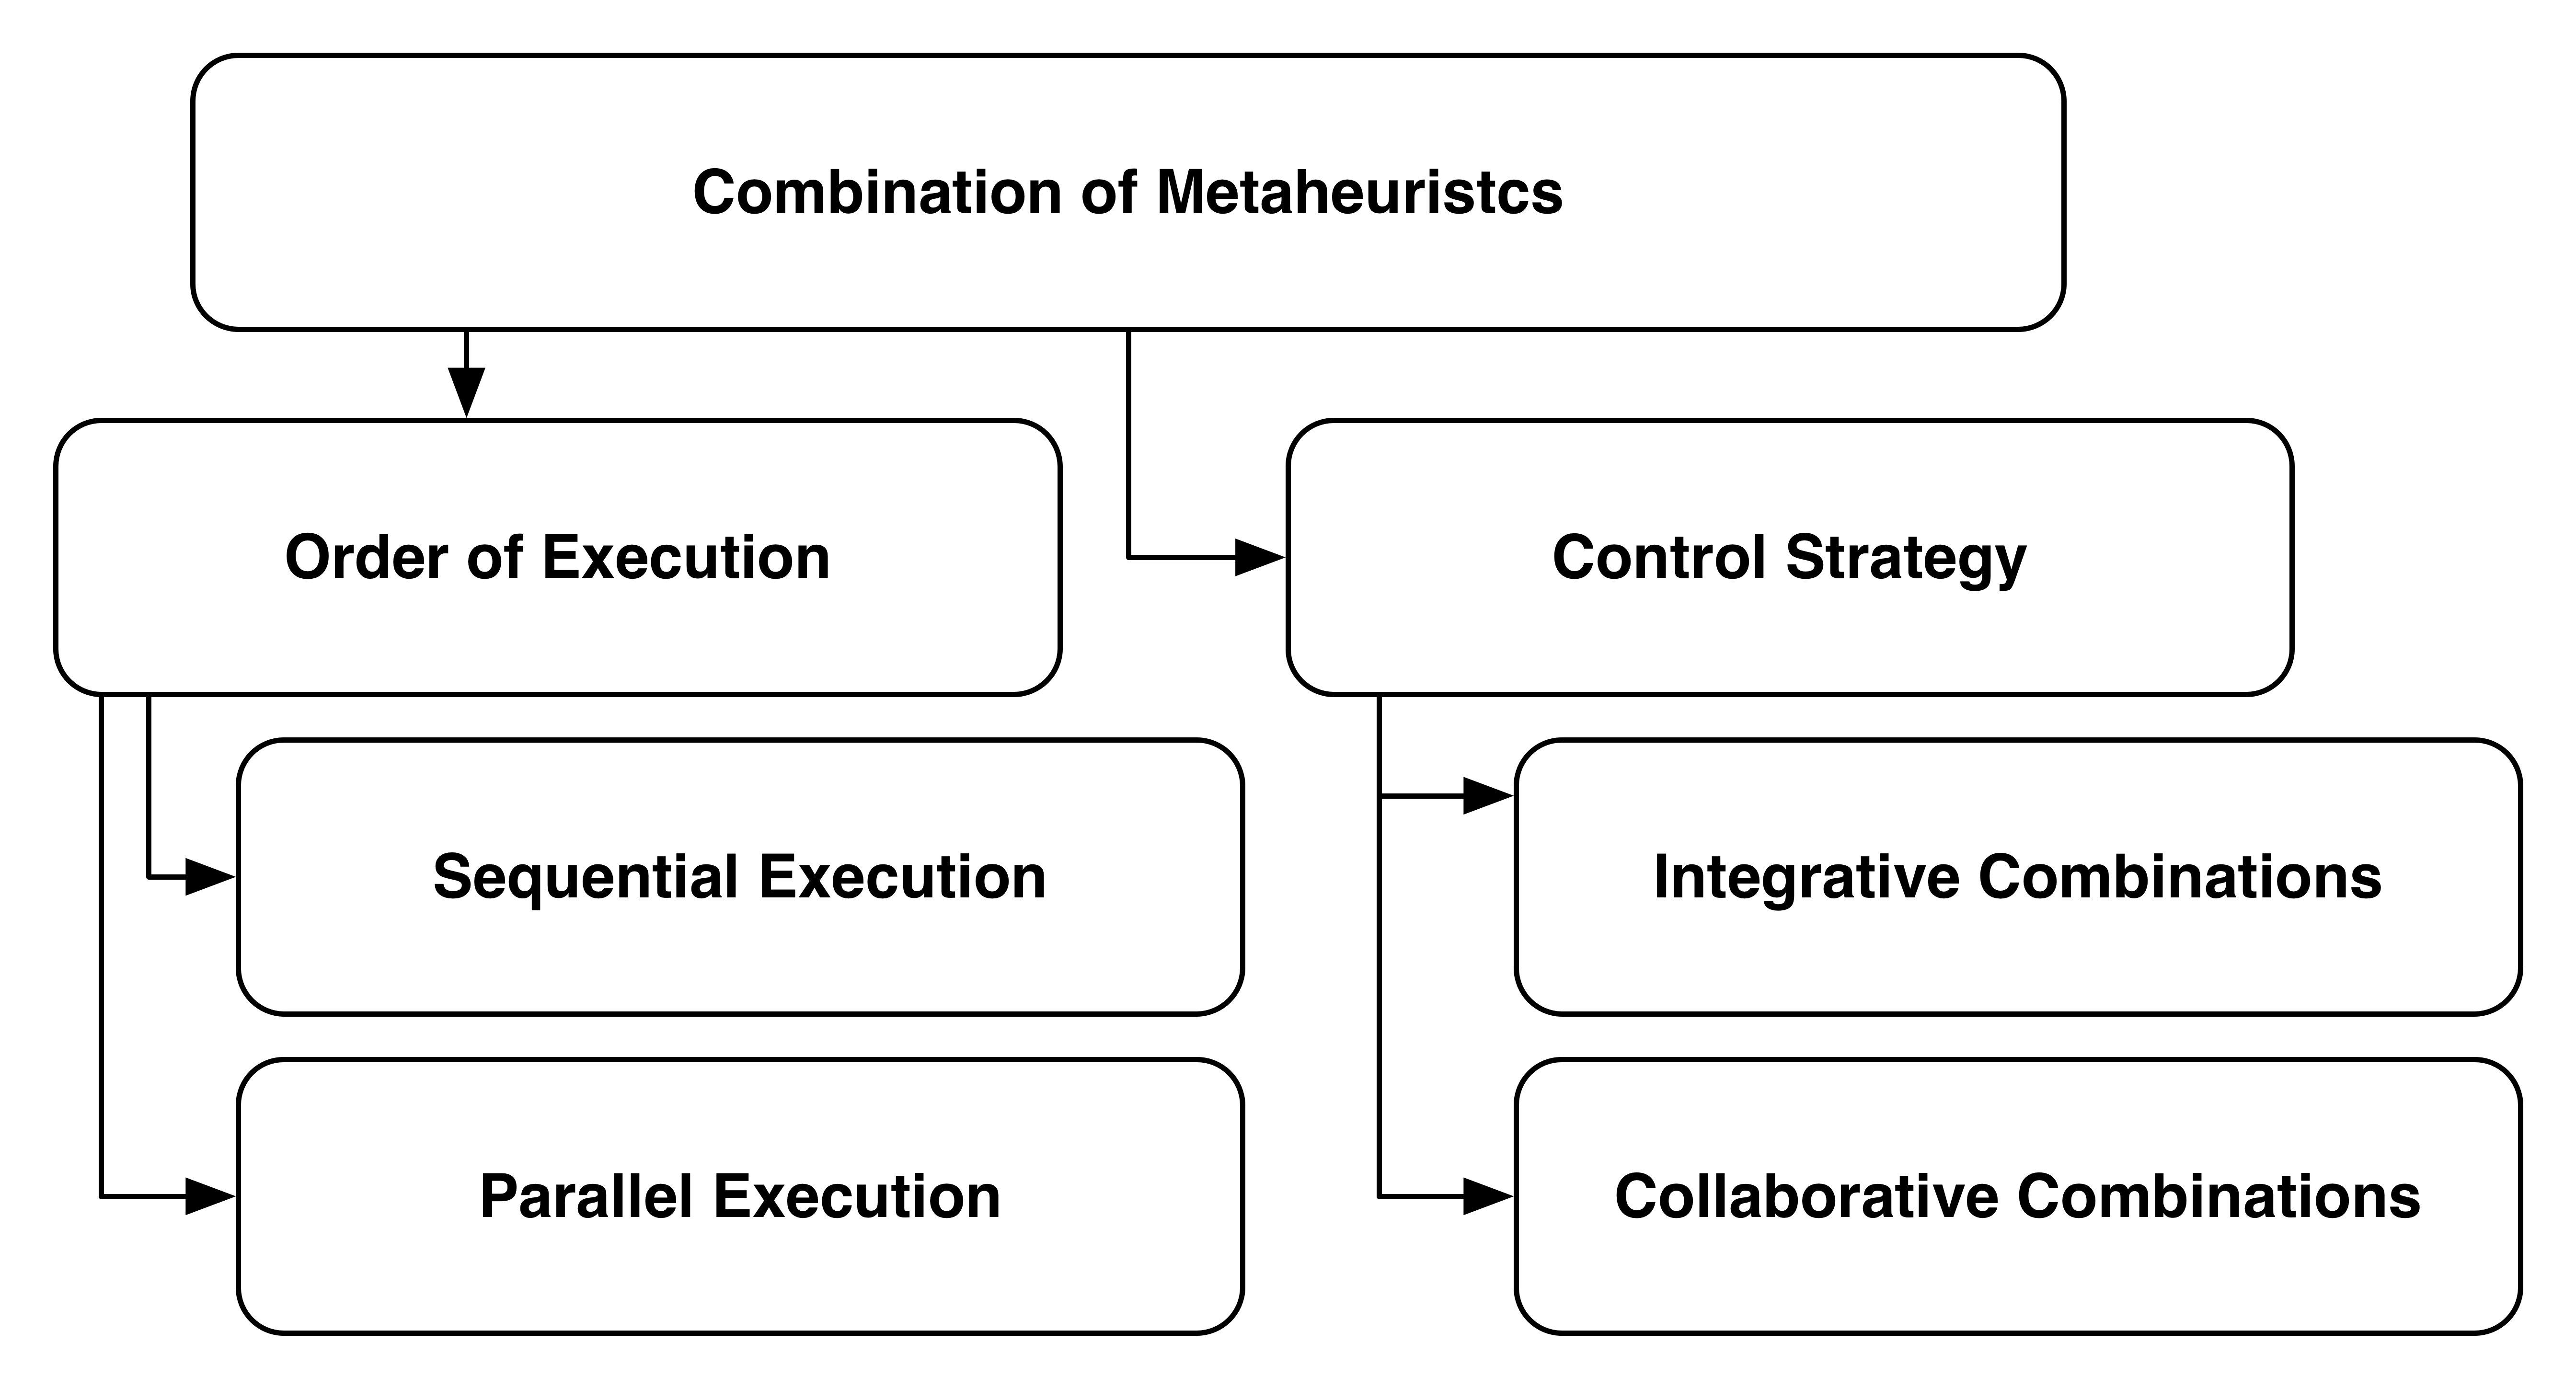
\includegraphics[width=1\textwidth]{./images/metaheuristc2.png}
\caption{Categories of metaheuristc combinations \cite{Puchinger2005} }
\label{fig:metaheuristc}
\end{figure}

Collaborative combinations use an approach where the algorithms exchange information, but are not part of each other. In this approach, algorithms may be executed sequentially or in parallel. 

One of the most popular ways of metaheuristic hybridization consists in the use of trajectory methods inside population-based methods. Population-based methods are better in identifying promising areas in the search space from which trajectory methods can quickly reach good local optima. Therefore, metaheuristic hybrids that can effectively combine the strengths of both population-based methods and trajectory methods are often very successful \cite{raidl2010metaheuristic}.


The work uses a type of collaborative combination with sequential execution with two trajectory methods (Tabu Search and Simulated Annealing) and Genetic Algorithms.

\section{Multi-Objective Optimization}

Many real optimization problems require optimizing multiple conflicting objectives with each other. There is no single optimal solution, but a set of alternative solutions. The objectives that have to be optimised are often in competition with one another and may be contradictory; we may find ourselves trying to balance the different optimisation objectives of several different goals \cite{Harman2010} \cite{el2014local}.

The image of all the efficient solutions for is called Pareto front or Pareto curve or surface. The shape of the Pareto surface indicates the nature of the trade-off between the different objective functions. An example of a Pareto curve is reported in Fig. \ref{fig:pareto1}. Multiobjective optimization methods have as main purposes to minimize the distance between the non-dominated front and the Pareto optimal front and find a set of solutions that are as diverse as possible. 

\begin{figure}[h]
\centering
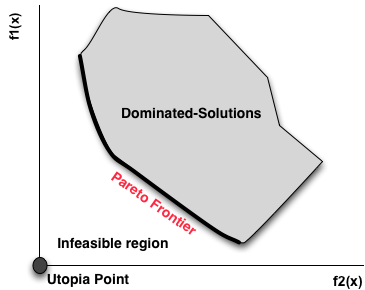
\includegraphics[width=0.4\textwidth]{./images/paretofront.png}
\caption{An mimization pareto front example}
\label{fig:pareto1}
\end{figure}

What distinguishes multi-objective EAs from singleobjective metaheuristics is how they rank and select individuals in the population. If there is only one objective, individuals are naturally ranked according to this objective, and it is clear which individuals are best and should be selected as
parents. In case of multiple objectives, it is still necessary to rank the individuals, but it is no longer obvious how to do this. Most people probably agree that a good approximation to the Pareto front is characterized by:

\begin{itemize}
\item  a small distance of the solutions to the true Pareto frontier,
\item  a wide range of solutions, i.e., an approximation
of the extreme values, and
\item a good distribution of solutions, i.e., an even
spread along the Pareto frontier.
\end{itemize}

Multi-objective metaheuristics rank individuals according to how much they contribute to the above goals.

\subsection{NSGA-II Multiobjective heuristics}

Deb et al.  proposed the NSGA II taking into account the need to reduce computational complexity in non-dominated classification, introduce elitism and eliminate subjectivity in the allocation of the sharing parameter \cite{Deb2000}. NSGA II (Non-dominated Sorting Genetic Algorithm II)  is a multiobjective algorithm, based on Genetic Algorithms  and that implements the concept of Dominance, that is, to classify the Total Population in fronts according to the degree of dominance. According to NSGA II, the individuals that are located on the first front are considered the best solutions of that generation, while in the last front are the worst. Using this concept, one can find more consistent results, points closer to the Pareto region, and that are better adapted to the type of problem. 

The NSGA algorithm II applies a fitness evaluation in an initial population (Figure \ref{fig:nsga2}- \ding{202} and \ding{203}). The population are ranked using multiple tournament selection, which consists of comparing two solutions (Figure \ref{fig:nsga2}- \ding{204}). In order to estimate the density of the solutions surrounding a particular solution in the population, the common distance between the previous solution and the posterior solution is calculated over each of the objectives. This distance serves as an estimate of the size of the largest cuboid that includes solution i without including any other solution of the population. A solution i wins another solution if:

\begin{itemize}
\item Solution i has a better rank, then $Rank_i$ <$Rank_j$.
\item Both solutions have the same rank, but i has a
Distance better than j, then $Rank_i$ = $Rank_j$ and $Distance_i$>$Distance_j$.
\end{itemize}

At the end of each analysis a certain group of individuals are classified as belonging to a specific category called the front and upon completion of the classification process all individuals will be inserted into one of the n fronts. Front 1 is made up of all non-dominated solutions. Front 2 can be achieved by considering all non-dominated solutions excluding solutions from front 1. For the determination of front 3, solutions previously classified on front 1 and 2 are excluded, and so on until all individuals have been Classified on some front.

After selection, recombination and mutation are performed as in conventional Genetic Algorithms (Figure \ref{fig:nsga2}- \ding{205}). The two sets (father and son of the same dimension) are united in a single population (dimension 2) and the classification is applied in dominance fronts. In this way, elitism is guaranteed preserving the best solutions (fronts not dominated) in the later population (Figure \ref{fig:nsga2}- \ding{207}).

However, not all fronts can be included in the new population. Thus, Deb et al. proposed a method called crowd distance , which combines the fronts not included in the set, to compose the last spaces of the current population, guaranteeing the diversity of the population \cite{Deb2000}. The NSGA-II algorithm creates a set of front lines, each front containing only non–dominating solutions. Within a front, individuals are rewarded for being ‘spread out’. The algorithm also ensures that the lowest ranked individual of a front still has a better fitness value than the highest ranked individual of the next front \cite{Harman2007}.







